\chapter{Method}
This chapter describes the material and method used for testing, the environment setup and the test cases that have been conducted. First, a survey for selecting the air quality monitors to be tested in this research are introduced. Then, the method for creating the environment, carrying out the tests, and analyzing the results are presented in a method tree and explained in details.  

\section{Air Quality Monitor Selection Survey}
To select the air quality monitors to use in this thesis, the problem description and research questions have been used as a reference. In order to answer the RQs, the air quality monitors need to be manufactured from different vendors. To find the specific \gls{AQM}s to use in this research, several online sources were used and compared. As this research is conducted by NTNU Gjøvik in Norway, it is also preferable that the devices are bought and available in Norwegian stores or webpages. The devices chosen should also be popular and easy accessible for any user. 

It exists many solutions that integrate air quality monitors within other devices, but as this thesis aims to investigate what private information is possible to infer from an air quality monitor, the devices should only have air quality monitoring functionality.  Considering these factors, the following criteria are made out to select the devices:
\begin{itemize}
    \item The devices are manufactured from different vendors.
    \item The devices communicates over \gls{Wi-Fi}.
    \item The devices are available for any user.
    \item The devices only monitors indoor air quality.
    \item The devices are available in Norwegian stores.
\end{itemize}
Tibber \cite{Tibber} is a Norwegian power company that specializes in combining smart technology, as with \gls{IoT} devices, and live app representation of the power consumption and smart devices \cite{Tibber}.  Tibber has over 400,000 users in Northern Europe, which makes them a natural choice for many when integrating a smart home device to their environment \cite{TibberUsers}. On their website it is possible to buy several \gls{IoT} smart devices for our home. They recommend one \gls{AQM} which communicates over \gls{Wi-Fi}, Netatmo Smart Indoor Air Quality Monitor. Netatmo \cite{Netatmo} is a company that specializes in consumer technology. They have one indoor air quality monitor which uses four sensors to monitor the indoor air quality of an environment. The sensors are; humidity, \(CO_2\), noise and temperature. 

Elkjøp \cite{Elkjøp} and Komplett \cite{Komplett} are two of Norway's biggest electrical stores with a wide range of different smart home devices both in store and online. Its therefore a natural choice when users are looking for any electronic devices including smart devices. When searching for "Air Quality Monitors" on their web pages, Elkjøp shows 4 different vendors and Komplett 8 different vendors. Both vendors lists Netatmo Healthy Home coach, which is already chosen. A part from this both Elkjøp and Komplett also recommends Mill Sense. Mill \cite{Mill} is a Norwegian company that manufactures and sells products for indoor climate and heating, with the goal of developing devices that fits the indoor interior environment. They offer one air quality monitor called Mill Sense which communicates over \gls{Wi-Fi}. The sensors integrated are \(eCO_2\), humidity, temperature and \gls{TVOC}.

When sorting the devices on client reviews on Komplett, the highest ranking manufacturer of air quality monitors is Nedis SmartLife \cite{Komplett}. Nedis \cite{Nedis} is an electronic company with the goal of making electronic-related solutions based on the newest technology. They have different solutions for air quality monitors, but the one that communicates over \gls{Wi-Fi} is called Nedis SmartLife Air Quality Monitor WiFi. This device monitors \(CO_2\), HCHO, humidity, temperature and VOCs. 

This research will consists of air quality monitors from the selected three different vendors. The devices only works as air quality monitors and they have different sensors. The chosen devices from the survey are represented in Table \ref{tab:AQMSurvey}. 

\begin{table}[H]
    \centering
    \caption{Air quality monitor devices selected for this research}
    \begin{tabular}{| p{1.5cm} | p{5.5cm} | p{3cm} | p{2cm} |} 
        \hline
        Netatmo & Smart Indoor Air Quality Monitor & WiFi & \(CO_2\) \newline Noise \newline Humidity \newline Temperature \\
        \hline
        \textbf{Vendor} & \textbf{Air Quality Monitor} & \textbf{Communication protocol} & \textbf{Sensors} \\
        \hline
        Mill & Sense Smart Climatesensor & WiFi & \(eCO_2\) \newline Humidity \newline Temperature \newline \gls{TVOC} \\
        \hline
        Nedis & SmartLife Air Quality Monitor & WiFi & \(CO_2\) \newline HCHO \newline Humidity \newline Temperature \newline VOC \\
        \hline

    \end{tabular}
    \label{tab:AQMSurvey}
\end{table}

\subsection{Netatmo Smart Indoor Air Quality Monitor}
The Netatmo Smart Indoor Air Quality Monitor entails 4 different sensors: humidity, \(CO_2\), noise and temperature. It can be integrated with several smart indoor air quality monitor devices installed in users home, using HomeKit. It communicates over WiFi to its own app called \textit{Healthy Home Coach}. Figure \ref{fig:Netatmo} shows Netatmo Smart Indoor Air Quality Monitor and its corresponding application, Healthy Home Coach. 
\begin{figure} [H]
    \centering
    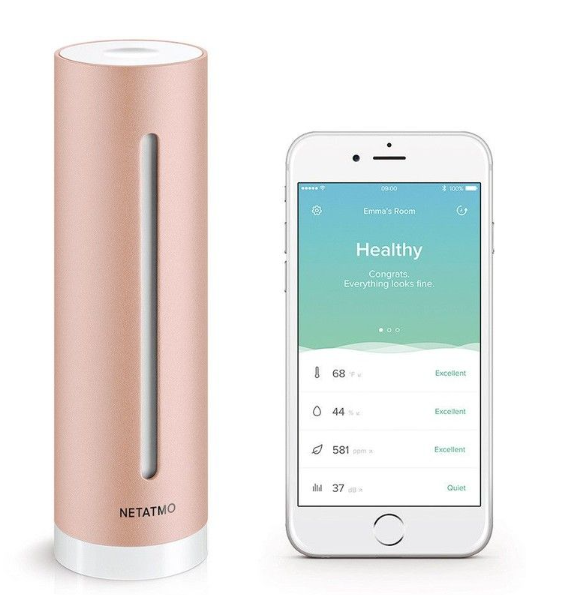
\includegraphics[width=0.4\textwidth]{figures/Netatmo.png}
    \caption{Netatmo Smart Indoor Air Quality Monitor and corresponding application Healthy Home Coach \cite{NetatmoDevice}}
    \label{fig:Netatmo}
\end{figure}

The Netatmo Smart Indoor Air Quality Monitor sends notifications to the user's application when the device sense high temperature, \(CO_2\), humidity or noise and low temperature or humidity. These are default enabled, but can be turned off by the user. The values cannot be changed, but are stated by Netatmo in the application. The unit displays live readings to the user, together with a graphical view of values over a longer period of time. When first installed, the device needs at least 7 days to finish calibrating and read the environment values correctly. 

\subsection{Mill Sense Air Quality Monitor}
Mill Sense Air Quality Monitor measures the indoor air quality with 4 different sensors: humidity, \gls{TVOC}, temperature and \(eCO_2\) \cite{Mill}. The monitor communicates through Wi-Fi and connects its data to their application called \textit{Mill Norway}. It is possible to use Mill Sense together with other Mill units, such as heaters or air purifiers,  to change their values based on the sensor data from Mill Sense \cite{Mill}. Figure \ref{fig:MillSenseBoth} shows Mill Sense and its corresponding application, Mill Norway. 

\begin{figure} [H]
    \centering
    \begin{subfigure}{0.3\textwidth}
         \centering
         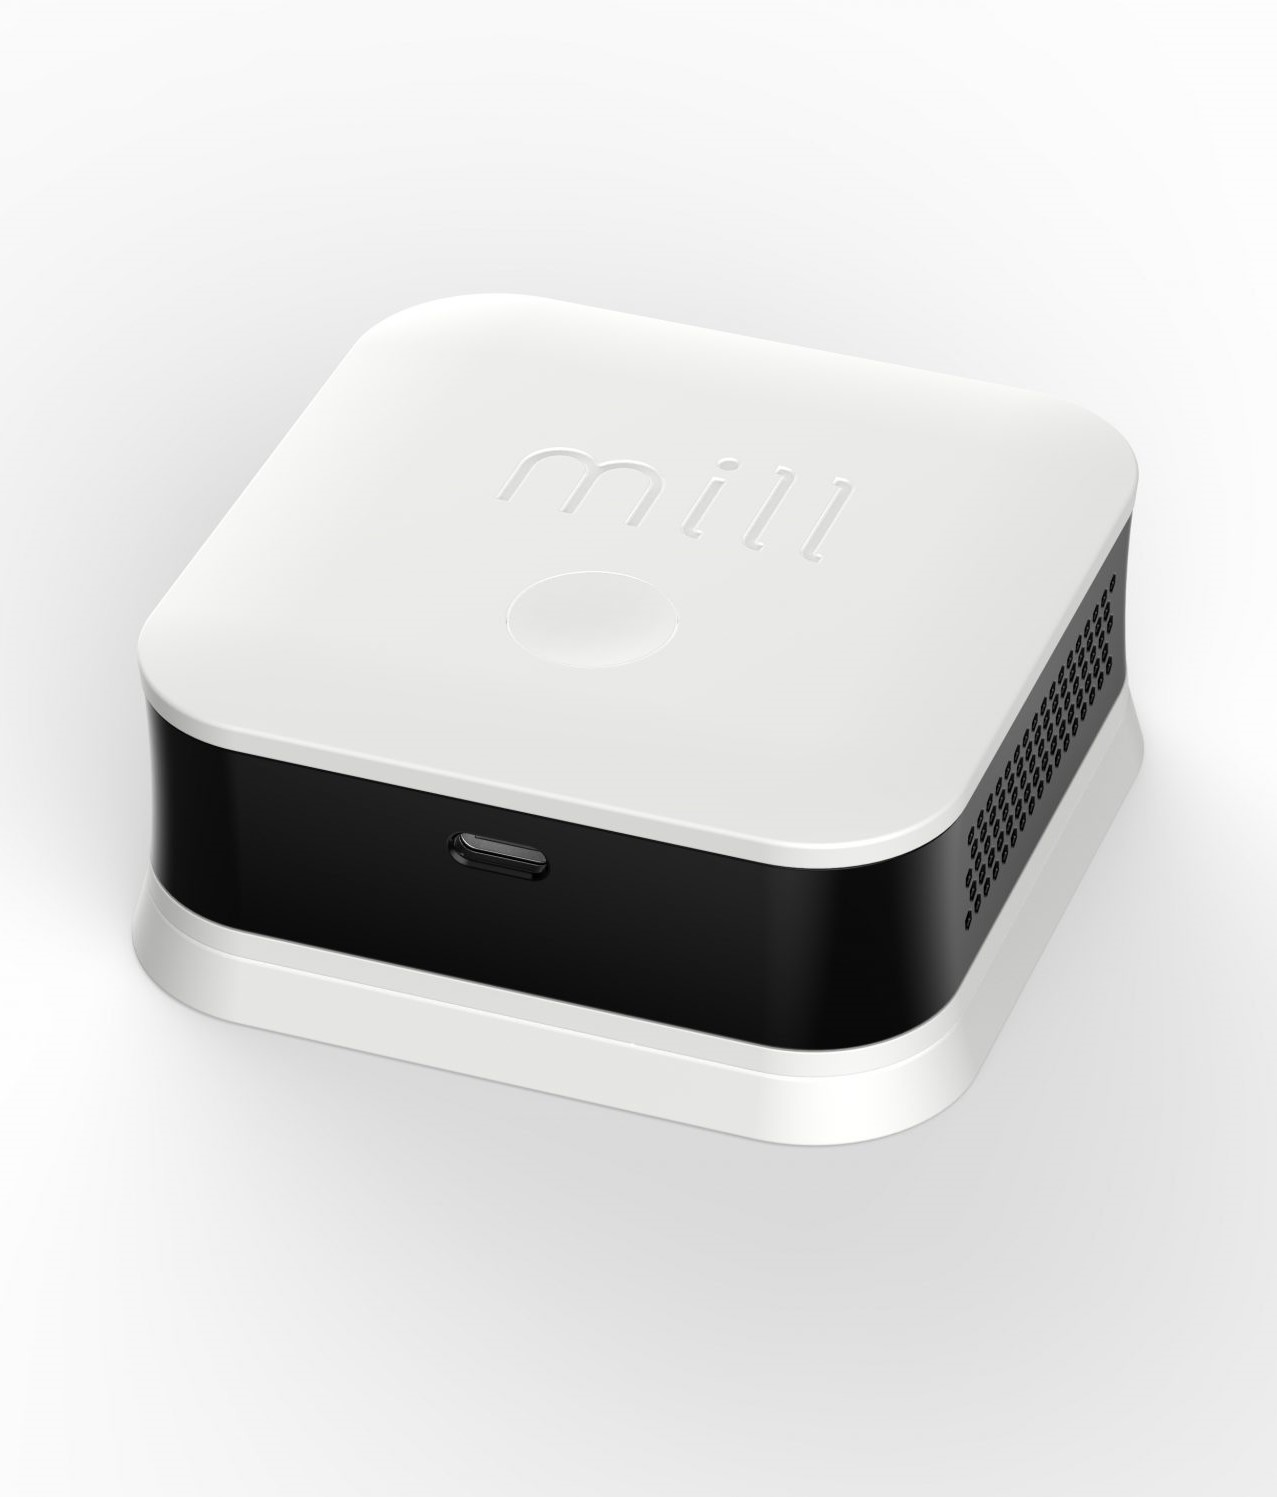
\includegraphics[width=1\textwidth]{figures/MillSense.jpg}
         \label{fig:MillSenseDev}
     \end{subfigure}
     \hspace{2cm}
    \begin{subfigure}{0.3\textwidth}
         \centering
         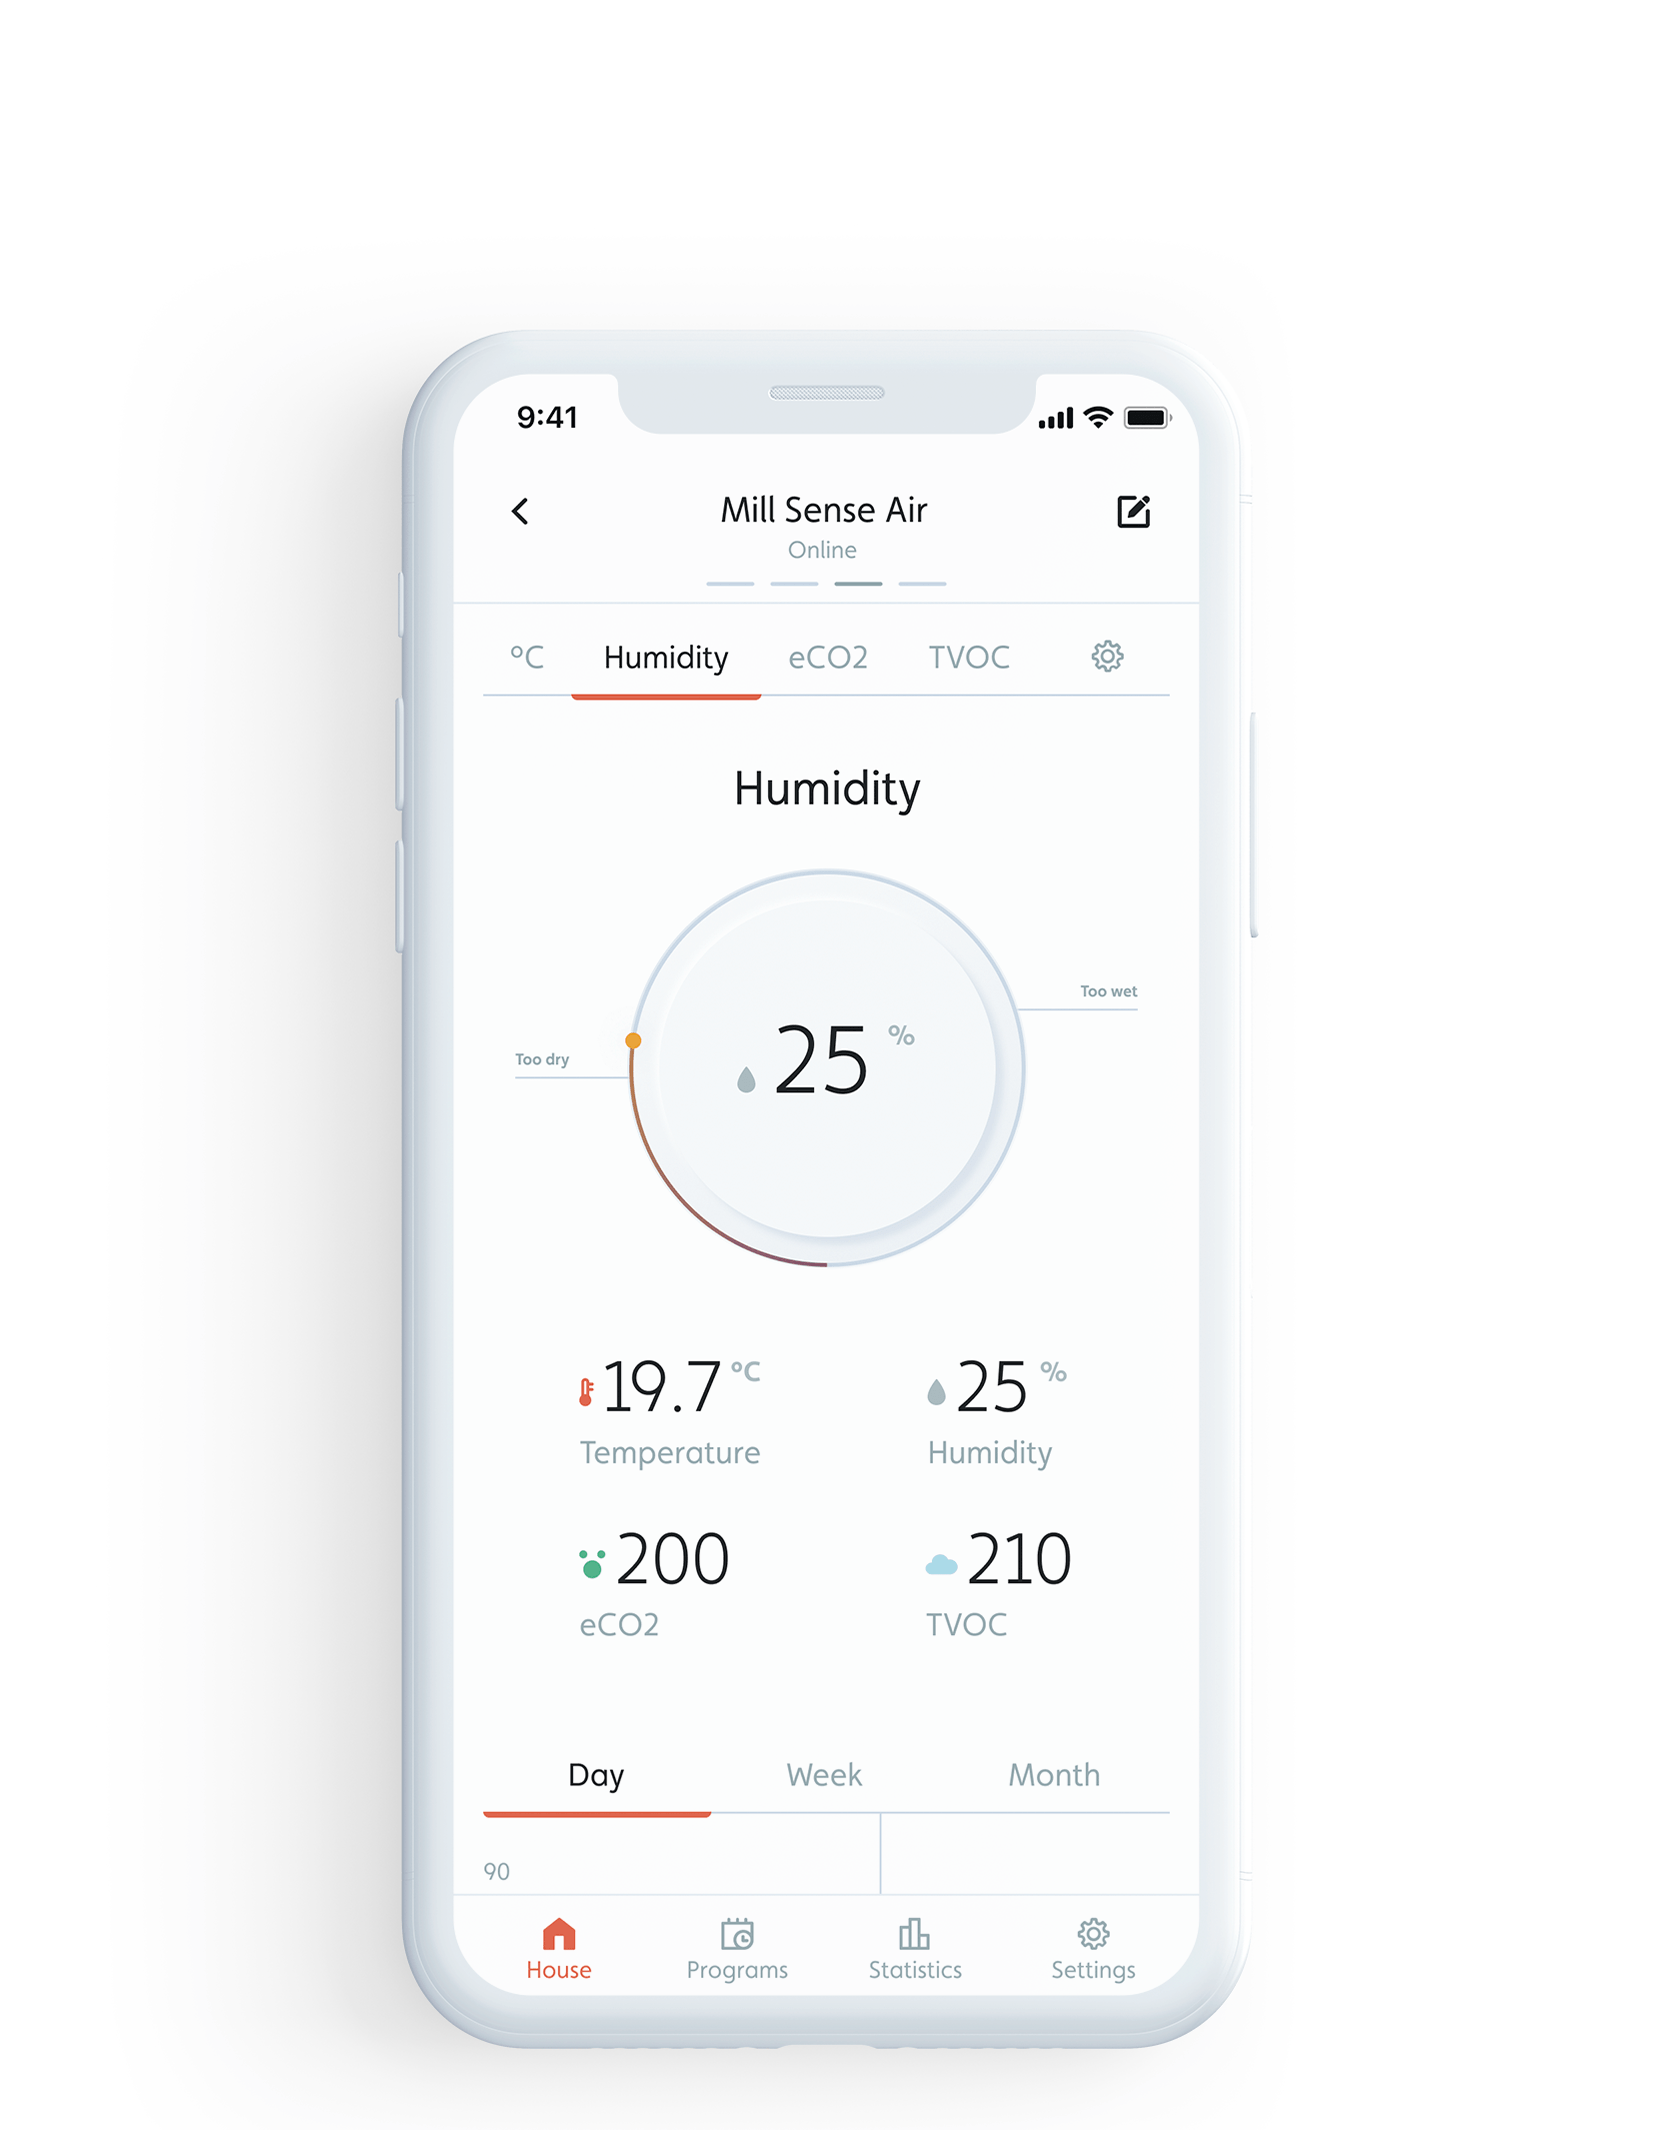
\includegraphics[width=1\textwidth]{figures/MillSenseApp.png}
         \label{fig:MillSenseApp}
     \end{subfigure}
     \hfill
        \caption{Mill Sense and corresponding application Mill Norway \cite{MillSense}}
        \label{fig:MillSenseBoth}
\end{figure}

The \gls{AQM} does not need power to stay connected and can be placed in any preferred room. The application does not provide notifications to users of threshold levels, but displays the current levels in the app together with graphs that shows variations back in time. Instead of sending notifications to a users phone, the device shows different light responses on the physical unit. These threshold values can be customized. The sensor data collected from the environment is sent to the cloud and back to the users app. It is possible to choose at what time interval the device will send sensor data, from every minute to every hour. When the unit is turned on for the first time and installed in the environment, the device needs at least 5 days to calibrate its sensors. 

\subsection{Nedis SmartLife Air Quality Monitor}
Nedis SmartLife Air Quality Monitor has 3 different indoor \gls{AQM} sensors: humidity, temperature and VOC \cite{NedisDevice}. The monitor communicates over \gls{Wi-Fi} to the app, Nedis SmartLife. As Nedis sells several other smart devices, the unit can be integrated in a smart environment together with other devices. Figure \ref{fig:NedisBoth} shows Nedis SmartLife Air Quality Monitor and its corresponding application, Nedis SmartLife. 
\begin{figure} [H]
    \centering
    \begin{subfigure}{0.3\textwidth}
         \centering
         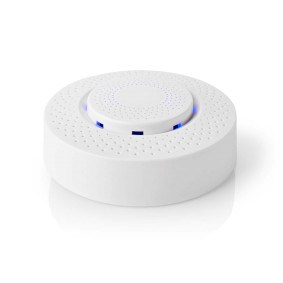
\includegraphics[width=1\textwidth]{figures/NedisDevice.jpg}
         \label{fig:NedisApp}
     \end{subfigure}
     \hspace{1cm}
      \begin{subfigure}{0.3\textwidth}
         \centering
         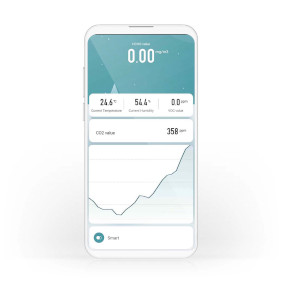
\includegraphics[width=1\textwidth]{figures/NedisApp.jpg}
         \label{fig:NedisDev}
     \end{subfigure}
     \caption{Nedis SmartLife and corresponding application Nedis SmartLife \cite{Nedis}}
     \label{fig:NedisBoth}
\end{figure}

Nedis SmartLife does not have notifications enabled default, but it can easily be set and customized by the user. Every sensor reading from the device can be set to notify whether levels are too high or too low. The readings on the app shows live data as well as a graphical view of previous readings. For setup and calibration in an environment, Nedis does not specify any calibration time.  

\section{Method Tree}
This research is structured in six different main activities, shown in Figure \ref{fig:MethodTree}:

\begin{figure} [H]
    \centering
    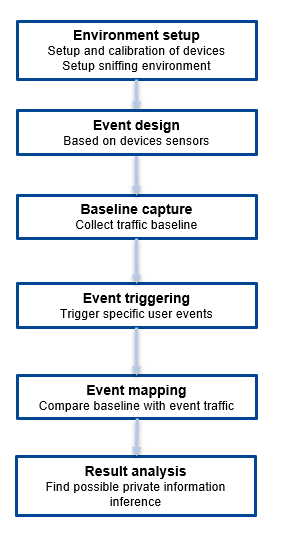
\includegraphics[width=0.4\textwidth]{figures/MethodTree.png}
    \caption{Method tree}
    \label{fig:MethodTree}
\end{figure}
\subsection{Environment Setup}
The first main activity is to set up the environment with both hardware and software correctly configured. First, the air quality monitors need to be functioning in the environment. Then a sniffer will be installed and tested to capture traffic sent to and from the devices. After this, the capturing and analysis platform is setup to store, process and analyze the data captured from the sniffer. On this platform, software designed to capture the necessary data needs to be installed and configured.  
\\\\
\textbf{Air Quality Monitors}\\
The \gls{AQM}s need to be installed, connected to their app and calibrated. The devices were installed and connected to the app as explained in the user manual attached to the devices. It is desirable that the air quality monitors gives notifications when a certain threshold value is met. However, for Mill Sense it is not possible to set notifications, but Nedis SmartLife and Netatmo Smart Indoor Air Quality Monitor were set with the same threshold values for notifications. For Mill Sense the interval for sending sensor data to the application were set to every minute. The \gls{MAC} addresses for the air quality monitors can all be found in their corresponding apps, since identifying and discovering the devices are out of scope for this thesis. 

Table \ref{tab:AQMSetup} describes each \gls{AQM}, their \gls{MAC} address and which sensor values triggers the devices to send notifications to the users phone. For the rest of this thesis, the devices will only be referenced with their manufactures name; Netatmo, Mill and Nedis, to simplify the presentations. 
 
\begin{table}[H]
    \centering
    \caption{MAC-address and notification threshold values for each AQM}
    \begin{tabular}{| p{3.5cm} | p{3.5cm} | p{5cm} |} 
        \hline
        \textbf{Air Quality Monitor} & \textbf{\gls{MAC} Address} & \textbf{Notification threshold values} \\
        \hline
        Netatmo & 70:EE:50:91:06:DE & \(CO_2\) > 1150 ppm \newline Noise > 62db \newline Humidity < 30\% \newline Humidity > 60\% \newline Temperature < 17 \degree C \newline Temperature > 26 \degree C \\
        \hline
        Mill & B8:F0:09:B3:B3:78 & N/A \\
        \hline
        Nedis & 2C:F4:32:29:36:DC & \(CO_2\) > 1000 ppm \newline Humidity < 30\%  \newline Humidity < 50\% \newline Temperature < 15 \degree C \newline Temperature > 25 \degree C \newline VOC > 99.9 ppm\\
        \hline
    \end{tabular}
    \label{tab:AQMSetup}
\end{table}

\noindent
\textbf{Sniffer}\\
In order to collect all \gls{Wi-Fi} traffic within the environment, a network sniffer was configured. The sniffer needs to be able to connect to the system were the packet capturing will take place and be set in monitoring mode. It exists a wide variety of available \gls{Wi-Fi} sniffers online, but the selected sniffer in this research is the TP-Link TL-WN722N. 

\begin{figure} [H]
    \centering
    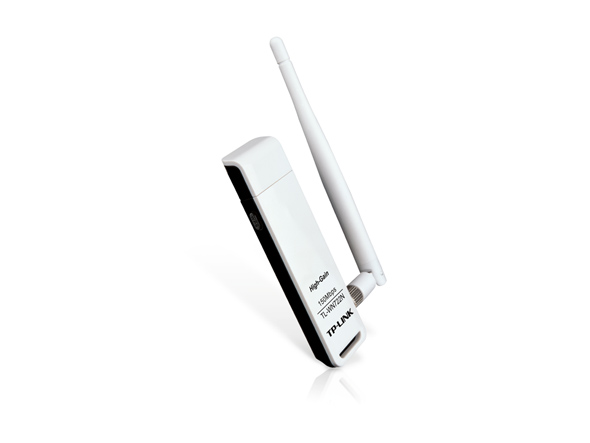
\includegraphics[width=0.5\textwidth]{figures/Sniffer.jpg}
    \caption{The \gls{Wi-Fi} sniffer selected in this research: TP-Link TL-WN722N \cite{Sniffer}}
    \label{fig:Sniffer}
\end{figure}

To set the device in monitoring mode, the is sniffer first plugged into a system and then the following four commands were applied:

\begin{verbatim}
    sudo ifconfig wlan0 down
    sudo iwconfig wlan0 mode monitor
    sudo ifconfig wlan0 up
    sudo iwconfig
\end{verbatim}

Note that wlan0 was the assigned wlan for the device when it was plugged it into the environment. The specific wlan addressed to the sniffer can vary from system to system so it needs to be checked with the device plugged into the system. When the sniffer is configured in monitoring mode, the device is able to collect all \gls{Wi-Fi} traffic within its own signal range. In this way, the sniffer will be able to collect the traffic sent to and from the \gls{AQM}s installed in the environment. To verify that the sniffer is collecting traffic on the network, Wireshark were used with the corresponding wlan, wlan0, as capturing interface. 
\\\\
\noindent
\textbf{Platform}\\
To collect data and store it from the devices, an operating system running on a hardware component with the possibility to connect the sniffer were setup. In this thesis, Raspberry Pi Model 3 B+ were chosen as it can continuously be powered on to capture traffic over longer periods of time. The Raspberry Pi was installed with Kali Linux version 2022.3, installed from \cite{KaliLinux}, which was beneficial as it includes all the needed software to capture the traffic and is compatible with the TP-link sniffer. As the analysis will be conducted on another computer, WinSCP were used to export the files from the Raspberry Pi over the network, downloaded from \cite{WinSCP}. Figure \ref{fig:Environment} shows a logical overview of the setup of the environment.  

\begin{figure} [H]
    \centering
    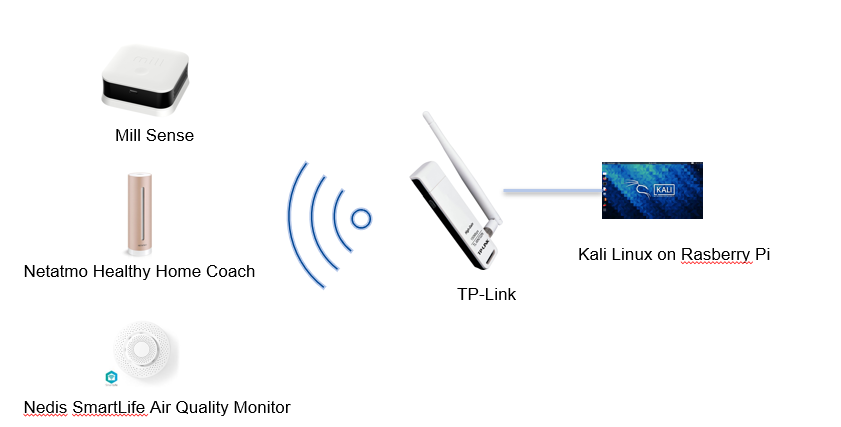
\includegraphics[width=1\textwidth]{figures/Environment.png}
    \caption{Environment setup with all devices \cite{MillSense}, \cite{NetatmoDevice}, \cite{NedisDevice}, \cite{Sniffer}, \cite{KaliLinux}}
    \label{fig:Environment}
\end{figure}

\textbf{Tshark}\\
In order to store and process the traffic that the sniffer collects, a monitoring software was used. Tshark \cite{Tshark} is an open-source network packet analyzer and were used to store packets. Tshark can be run from the command line interface and has the possibility of using capture filters based on a number of parameters, such as addresses, duration or size. In order to store the packets captured, tshark was run with the option of writing its results to an output file rather than directly in the command-line, as it does default. The packets collected in the output file by tshark are possible to open and analyze in Wireshark. 

To store packets from all the three air quality monitors, tshark was run from three different terminals with corresponding filter to the devices. The options of the command are explained in Table \ref{tab:tshark}.

\begin{table}[H]
    \centering
    \caption{Tshark command options used to capture traffic}
    \begin{tabular}{|l|l|}
    \hline
    \textbf{Filter option} & \textbf{Usage}                        \\ \hline
    tshark                 & Initialize tshark                     \\ \hline
    -i                     & Interface to be used                  \\ \hline
    -f                     & Capturing filter                      \\ \hline
    -w                     & Output file to store captured packets \\ \hline
    \end{tabular}
    \label{tab:tshark}
\end{table}

\begin{verbatim}
Netatmo:
    tshark -i wlan0 -f "ether.host == 70:EE:50:91:06:DE" -w 
    "\\Documents\Netatmo"
Mill:
    tshark -i wlan0 -f "ether.host == B8:F0:09:B3:B3:78" -w 
    "\\Documents\Mill"
Nedis:
    tshark -i wlan0 -f "ether.host == 2C:F4:32:29:36:DC" -w 
    "\\Documents\Nedis"
\end{verbatim}


\subsection{Event Design}
In order to infer user behaviour from the devices, several test cases were designed. As the \gls{AQM}s are installed and monitors the home environment at all times, the test cases are not limited in time or place in the house as they can be moved. 

Looking at the different sensors and how they can be affected is important for understanding which user behaviour can possibly change traffic pattern. The sensors from all the devices combined are; \(eCO_2\), \(CO_2\), humidity, temperature, \gls{TVOC}, \gls{VOC}, HCHO and noise. Some of the sensors will be affected by the same actions, so they will be categorized together. The following significantly different categorized sensors will be used: \(CO_2\), humidity, temperature, VOC and noise. Examples of user behaviour in a home that affects the different sensors are:
\begin{itemize}
    \item $\mathbf{CO_2:}$ People or animals present, cooking, windows open
    \item \textbf{Humidity:} Windows open, showering
    \item \textbf{Temperature:} People or animals present, windows open, fireplace lit
    \item \textbf{VOC:} Cooking, burning candles
    \item \textbf{Noise:} Many people present, playing music or TV
\end{itemize}

Several of the proposed user behaviours will affect not only one, but several sensors. However, it is more beneficial to focus on routines that users do every day to be able to see a pattern of a household instead of looking at one specific action that users may not do regularly. It is also important to notice that in order to infer private information from network traffic, the test cases needs to change the sensor values by some degree. Therefore, repetitive behaviour that has the possibility to change the threshold values are chosen initially. 

The three different routinely test cases chosen are \textbf{cooking}, \textbf{showering} and \textbf{windows open at night}. Cooking is the most routinely behaviour in a home where dinner is normally made every day. The next test case is showering as this is a routine behaviour and will affect the sensors, particularly humidity and temperature in the bathroom. Showering can be routinely done at very different times, but evening showers are used in this case. Windows in a home can be open at several times, however, having a window open every night while sleeping can be common and should drastically change the indoor temperature and possibly humidity. Especially since the testing will be carried out during winter time in Norway. This is also a test that will last longer than the other two tests and can possibly give another aspect to the research. 

Another test case that can be interesting to see if changes the traffic patterns when a user are home or not. Therefore, a weekend test will be carried out. The sniffer will gather traffic from several weekends when the user is present in the home environment and compare it to when the user is away for the weekend and look at the differences.

The four test cases chosen are three routine test cases and one test case not based on routines. It is important to understand that the privacy of the different test cases are different. Knowing whether a user is cooking or showering are defined as the two test cases with the least dangerous private information exposed, while window open at night can rather indicate that a user is sleeping and the home environment is not watched. The private information exposed from the weekend test, is the most dangerous if revealed since it will indicate if a user is gone and therefore not in control of the home environment.

\subsection{Baseline Capture}
To be able to distinguish the events in the \gls{Wi-Fi} traffic, it is necessary to capture and analyze traffic from the devices when they are not affected by any events. This is necessary to understand what normal traffic from the devices is, like presented in \cite{NetAna}. During the baseline capture, the devices were installed and calibrated in the environment. All notifications that will be enabled during the event triggering were enabled. The devices were reachable through their app and communicate in their own pattern. The baseline capture was on-going for several days to ensure enough data and traffic was collected. During this capture, the devices were placed in the inner hallway of the apartment. It would have been ideally to have a baseline from each room of where the test cases will be located, but due to time constraints, they were placed in a room binding all the other rooms together. See Figure \ref{fig:Apartment} for an overview of the environment.

\subsection{Event Triggering}
In this activity, traffic from the devices were captured while the events were triggered. The routine events are each triggered 10 times and traffic from at least 1 hour before and after the event were captured to see the changes in traffic both before and after the events. Weekend testing were conducted in the course of 14 weekends, resulting in collected traffic from 7 weekends at home and 7 weekends gone. 

Table \ref{tab:TestCases} gives an overview of the time of day when each test case was carried out and in which room the devices were placed for the tests. 
\begin{table}[H]
    \centering
    \caption{Overview of test cases with timings and location}
    \begin{adjustbox}{width=1\textwidth}
    \begin{tabular}{| p{5cm} | p{5cm} | p{3cm} |} 
        \hline
        \textbf{Test Case} & \textbf{Time of day} & \textbf{Room} \\
        \hline
        Cooking & After work: 4pm to 5pm & Kitchen \\
        \hline
        Window open at night & At night: 11pm to 7am & Bedroom\\
        \hline
        Showering & Afternoon: 8pm to 9pm & Bathroom \\
        \hline
        Weekend tests & Friday: 4pm to Sunday: 11pm & Living room \\
        \hline
    \end{tabular}
    \end{adjustbox}
    \label{tab:TestCases}
\end{table}

As there is only one of each device and the tests are in different rooms, the devices were moved to the corresponding room before each test. The devices were placed in the environment for at least 1 hour before each test starts to ensure that the value changes between the room will be as equalized as possible. The exact times for when cooking, open window and showering took place were be logged so it is possible to look for changes at that time. 

Figure \ref{fig:Apartment} shows an overview of the apartment layout, hereby called \textbf{the environment}, where the test cases and baseline were captured from. The different rooms are marked and shows where the devices were placed during the different tests. 

\begin{figure}[H]
    \centering
    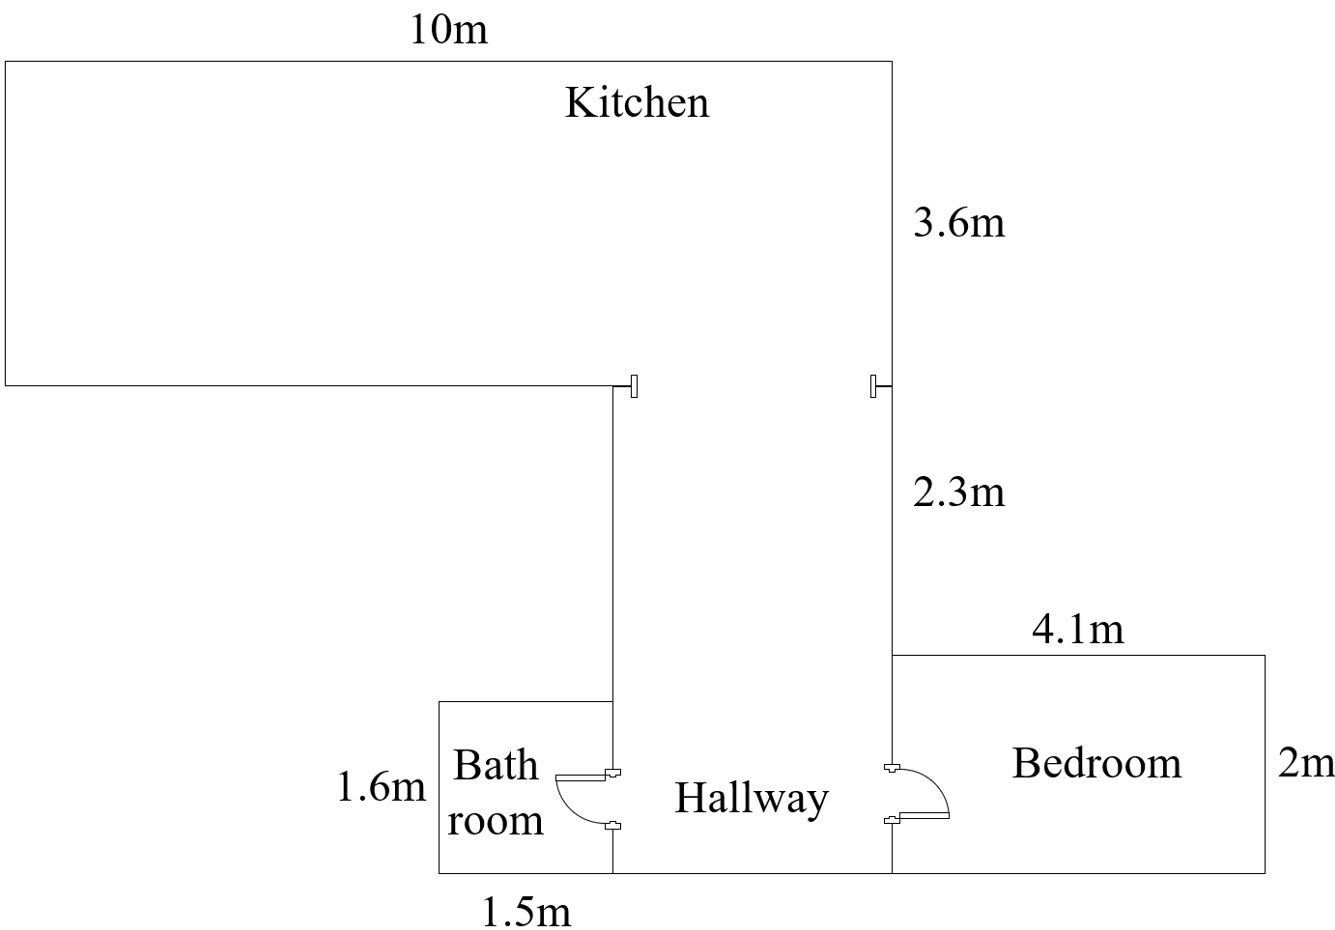
\includegraphics[width=0.7\textwidth]{figures/Apartment.png}
    \caption{Overview of the environment for the test cases and baseline capturing. Cooking in the kitchen, showering in the bathroom, window open at night in the bedroom and baseline and weekend tests in the hallway.}
    \label{fig:Apartment}
\end{figure}

\subsection{Event Mapping}
When the events had been carried out, a mapping was made to see if information could be inferred. Each event is presented both graphically and numerically with different calculations to compare. Each event were extracted from the corresponding tshark capture saved in the pcap output file. A separate pcap file for each event was made, with the timing of the specific event to see differences. 

\subsection{Result Analysis}
The last activity is to analyze the results from the tests performed. Each event has initially been evaluated and analyzed with the same general procedure. Figure \ref{fig:GeneralProcedure} shows an overview of the steps each event has been through. The results from each event are presented and explained in each subsection and in some cases, the general procedure has given insights to further analysis which is covered in the Evaluation and Analysis Results.

\begin{figure}[H]
    \centering
    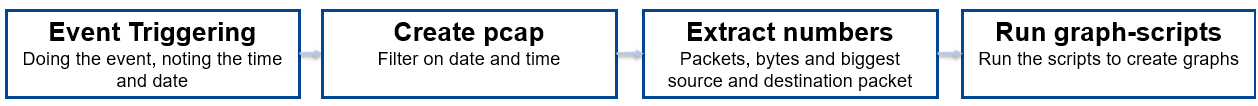
\includegraphics[width=\textwidth]{figures/GeneralProcedure.png}
    \caption{General procedure used to evaluate and analyze the test cases}
    \label{fig:GeneralProcedure}
\end{figure}

To be able to run analysis on the data gathered from the different \gls{pcaps} and present it in an understandable way, two different programs were used: Wireshark and python scripts in \gls{VS Code} with pyshark, a tshark library. Wireshark was used to extract numbers and calculations from the pcaps and \gls{VS Code} was used to generate graphs from event \gls{pcaps}.

When opening a pcap in Wireshark, several statistics are possible to extract. By choosing the option of "Capture File Properties", total number of packets and bytes in the capture file are shown and were extracted. The numbers from each pcap were noted down and used as event attributes to compare both the events to each other and to the baseline. Another value used to analyze the events where packet lengths. The biggest packet from each capturing were noted down to use for comparing and looking for patterns and changes during an event. 

In \gls{VS Code}, python was used as the programming language as it includes the library pyshark which can be used towards the tshark capture files. Four scripts with a number of different if statements were used to generate different graphs depending on system arguments passed to the script. The scripts were used to generate two graphs: one with number of bytes or packets per execution of event and one for the corresponding baseline event. The code is displayed in its whole in Appendices \ref{app:GraphsByBytes}, \ref{app:GraphsByPackets}, \ref{app:GraphsByBytes_BaselineEvents} and \ref{app:GraphsByPackets_BaselineEvents}, and in pseudo code beneath in Algorithm \ref{alg:GraphScript}. For each of the if statements, the same code block is included and are only shown once in Algorithm \ref{alg:GraphScript}. The graphs are all generated with bytes or packets per 2 seconds, where the y-axis is defined in the number of packets or bytes and the x-axis defined as time. The scripts uses parts from the scripts explained in \cite{GraphsInspiration}.

To create a file for each of the events, a time filter was applied to the pcaps and the remaining packets exported to a separate pcap creating one pcap file per captured event. These can be opened in Wireshark or make a graph out of to analyze each specific event. The time filter used followed the following format:

\begin{itemize}
\item \textbf{Format:} frame.time >= "Month Date, Year "Time"" \&\& frame.time <= "Month Date, Year "Time""//
\item \textbf{Example:} frame.time >= "Jan 08, 2023 "19:30:00"" \&\& frame.time <= "Jan 08, 2023 "20:40:00""
\end{itemize}

Table \ref{tab:SystemArgumentsScripts} displays the different system arguments passed to the scripts to create the graphs and which values the arguments expect. 

\begin{table}[H]
    \centering
    \caption{Overview of system arguments for scripts}
    \begin{adjustbox}{width=1\textwidth}
    \begin{tabular}{l|l|l|}
        \cline{2-3} & \textbf{Description} & \textbf{Values}\\ \hline
        \multicolumn{1}{|l|}{\textbf{Argument 1}} & Name of device & \begin{tabular}[c]{@{}l@{}}Netatmo\\ Mill\\ Nedis\end{tabular} \\ \hline
        \multicolumn{1}{|l|}{\textbf{Argument 2}} & Which packets to include & \begin{tabular}[c]{@{}l@{}}Inbound packets and bytes\\ Outbound packets and bytes\\ Inbound and outbound packets and bytes\end{tabular} \\ \hline
        \multicolumn{1}{|l|}{\textbf{Argument 3}} & Type of event & \begin{tabular}[c]{@{}l@{}}Cooking\\ Shower\\ Window\\ Weekend\\ Baseline\end{tabular} \\ \hline
        \multicolumn{1}{|l|}{\textbf{Argument 4}} & Maximum value for y-axis, in bytes or packets & <Numeric value> \\ \hline
    \end{tabular}
    \end{adjustbox}
    \label{tab:SystemArgumentsScripts}
\end{table}

\begin{algorithm}[H]
\caption{Script for generating graphs}\label{alg:GraphScript}
    \begin{algorithmic}[1]
        \For{Each date of event} \Comment{Graph\_function start}
            \State Extract the packets from the right pcap
            \For{Each packet in pcap}
                \State Extract packet length in byte and time or add packet count to time
                \State Display graph
            \EndFor
        \EndFor \Comment{Graph\_function end}\\
        \If{Argument 2 is Outbound} \Comment{Set display filter to outbound traffic}
            \If{Argument 1 is Netatmo}
                \State Set display filter to "wlan.sa == Netatmo \gls{MAC} address"
            \ElsIf{Argument 1 is Mill}
                \State Set display filter to "wlan.sa == Mill \gls{MAC} address"
            \ElsIf{Argument 1 is Nedis}
                \State Set display filter to "wlan.sa == Nedis \gls{MAC} address"    
            \EndIf \\
        \ElsIf{Argument 2 is Inbound} \Comment{Set display filter to inbound traffic}
            \If{Argument 1 is Netatmo}
                \State Set display filter to "wlan.da == Netatmo \gls{MAC} address"
            \ElsIf{Argument 1 is Mill}
                \State Set display filter to "wlan.da == Mill \gls{MAC} address"
            \ElsIf{Argument 1 is Nedis}
                \State Set display filter to "wlan.da == Nedis \gls{MAC} address"  
            \EndIf
        \EndIf \\
        \If{Argument 3 is Shower} \Comment{Event if-cases start}
            \State Set the dates from when the events occurred 
            \State Graph\_function
        \ElsIf{Argument 3 is Cooking}
            \State Set the dates from when the events occurred 
            \State Graph\_function
        \ElsIf{Argument 3 is Window}
            \State Set the dates from when the events occurred 
            \State Graph\_function
        \ElsIf{Argument 3 is Weekend}
            \State Set the dates from when the events occurred 
            \State Graph\_function
        \ElsIf{Argument 3 is Baseline}
            \State Set the dates from when the events occurred 
            \State Graph\_function
        \EndIf \Comment{Event if-cases end}
    \end{algorithmic}
\end{algorithm}

To be able to look even further into differences in the traffic flow during an event and standard traffic, the baseline capturing were also extracted with the same time of day and duration as the corresponding events. To have the same start and finish time for the events and the baseline, timings for all executions of the events were used. The earliest starting time and the latest finish time for that event were used on every event, but also the baseline which was captured on different dates than the events. This results in both event and corresponding baseline pcaps possible to compare as they all have the same time interval. 

When these steps were finished for each execution of the events, graphs and calculations for the events were available to analyze. Average and standard deviation values were calculated for both the events and corresponding baseline \gls{pcaps}. To be able to conclude that there is a difference in traffic flow from when an event is ongoing, to standard traffic different measurements were used. The measurements are both calculations and graphical views and then compared to each other, using the same principles as proposed in \cite{SpyingonSmartHomes}. For calculations, the average value in packets and bytes for the baseline needed to be outside of the standard deviation for the event to conclude that there is possible to differentiate the events from other standard traffic.

The calculations for the routine tests also needed to be seen in context with the the traffic flows, as the calculations are not only made on traffic at the specific event time, but also includes traffic from a time period before and after the event. Since we do not expect the sensor values to change immediately when an event is triggered or finished, the traffic before is used as a reference to compare daily baseline traffic with the standby reference. The traffic after an event can still be affected by the sensor values since stabilizing the indoor air may take time. To be able to compare event and baseline calculations, the time before an event and the baseline needs to follow the same pattern. If the average value of the baseline were outside of the standard deviation of the event, and the traffic flow before an event were equal to the baseline traffic, then it was possible to conclude that the device exposed private information about the test case. 

The graphical measurement to analyze if there was a difference in traffic flow during the events, was if it was possible to see a constant difference in the traffic before and during an event. The baseline graphs were also used here to compare even more standard traffic, than the time period before the event and look further into if it was possible to see spikes or traffic flow changes during the events.The last numerical value analyzed is the biggest packet sent or received and can be used to see if there are bigger packets in the capture files while an event is ongoing, and if there are, look into if they are associated with the specific event time. This was included because we expect bigger packets to be sent or received by the device during an event to update sensor values or send notifications. The last numerical value analyzed is the biggest packet sent or received and can be used to see if there are bigger packets in the capture files while an event is ongoing, and if there are, look into if they are associated with the specific event time. This was included because we expect bigger packets to be sent or received by the device during an event to update sensor values or send notifications, which was also possible to find in \cite{PassiveInferenceIoT}. 

However, for the weekend test, baseline traffic were not used to compare. In this test, the weekends at home and the weekends gone are compared to each other to look at differences in the same way as explained for the routine behavioural tests. If the calculations showed that the average values for packets and bytes during a weekend gone was smaller than the standard deviation for a weekend at home, we can conclude that it is possible to infer this private information on the device. For this test, the graphical view of the traffic flow were used to strengthen the result if they gave the same result as the calculations. 